\subsection{Trackingsystem Microsot Kinect}\label{sec:kinect}
\vspace*{-.8cm}
\begin{figure}[H]
\centering
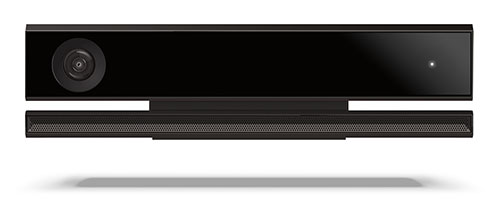
\includegraphics[width=.9\textwidth]{pictures/kinectimg.jpg}
\vspace*{-.5cm}
\caption{Frontalansicht der Kinect v2, Quelle: \cite{kinectimg}.}
\end{figure}
Die Kinect wurde in Versin 1 das erste Mal auf der E3 2009 in Los Angeles präsentiert, damals noch unter dem Namen \glqq{}Project Natal\grqq{} (siehe \cite{latimes}). Ziel war es, für Spiele der Xbox-Konsole von Microsoft den herkömmlichen Controller durch den Einsatz des gesamten Spielerkörpers zu ersetzen, nicht zuletzt, um damit ein breiteres Zielpublikum anzusprechen. Bereits zu diesem Zeitpunkt war geplant, unabhängigen Entwicklern die Verwendung und Programmierung des Systems zu ermöglichen (s. ebd.).\par 
Im Folgenden werden die technischen Spezifikationen der Kinect in ihrer aktuellen Version erläutert. Diese sind \cite{specs} entnommen. Die Kinect verfügt über eine Full-HD-Farbkamera und eine Infrarotkamera, die die Aufgabe des Tiefensensors erfüllt. Dieser ist mit 512 zu 424 Pixeln deutlich geringer aufgelöst. Der effektive Bereich ist laut Hersteller in einer Entfernung zwischen einem halben und 4,5 Metern. Die Kameras der Kinect liefern weiterhin maximal 30 Frames pro Sekunde. Weiterhin besitzt die Kinect ein Multi-Array-Mikrofon, mit dem Klang nicht nur aufgenommen, sondern auch hinsichtlich seiner Ausbreitung untersucht werden kann. Im Vergleich zu ihrer Vorgängerversion wurden vorwiegend Genauigkeitsverbesserungen vorgenommen, es kommt zu weniger Grundrauschen und die Objekterkennung ist generell stabiler und zuverlässiger. Mit der aktuellen Version können die Skelette von bis zu sechs Personen bei 25 Gelenkpunkten pro person vollständig getrackt werden (siehe Abbildung \ref{fig:Bild1}). Die zur Verfügung stehenden Gelenkpunkte lassen sich über die API des Kinect-SDK abfragen.
\begin{figure}[H] 
  \centering
  \begin{subfigure}{.6\textwidth}
  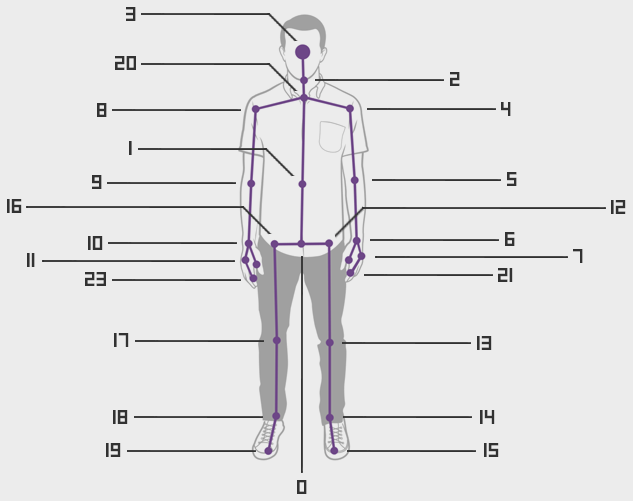
\includegraphics[width=\linewidth]{pictures/kinectskeleton-map2-1.png}
  \end{subfigure}\hfill
  \begin{subfigure}{.38\textwidth}
  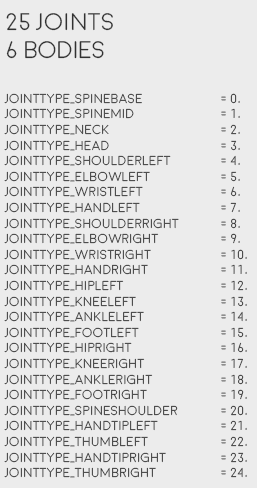
\includegraphics[width=\linewidth]{pictures/kinectskeleton-map2-2.png}
  \end{subfigure}
  \caption{\glqq{}Kinect V2 Joint ID Map\grqq{}, Gelenkpunkte die mit der Kinect getrackt werden können. Quelle (Ausschnitt): \cite{tracking2}}
  \label{fig:Bild1}
\end{figure}
Um die Tiefeninformation zu gewinnen, verwendet die Kinect in der zweiten Version ein sogenanntes Time-Of-Flight-Verfahren (hier und im Folgenden vgl. \cite{heise}). Grundlage ist die Gewinnung von 3D-Daten aus einem Kamerabild (in diesem Falle dem des Tiefensensors). Beim Time-Of-Flight-Verfahren wird für das ausgesendete Infrarotlicht gemessen, wie lange es braucht, um von der Objektoberfläche reflektiert zu werden und zurück zum Sensor zu gelangen. Beim Vorgänger, der Kinect-Version 1, wurde noch eine pseudorandomisiertes Muster auf die Szene projiziert und die Tiefeninformation daraus trianguliert (siehe \cite{gamasutra}). Ein Problem dieses Verfahrens ist die Forderung, für einen Punkt des Musters auch stets eine kleine Umgebung zu sehen, in der genug andere Lichtpunkte liegen, um eine Identifikation vorzunehmen. Der Time-Of-Flight-Ansatz der Kinect 2 besitzt diese Abhängigkeit nicht mehr. Eine weitere Verbesserung gegenüber der Kinect 1 ist das Vorhandensein eines eingebauten Umgebungslichtfilters: Wird ein Pixel von zu viel Licht aus dem sichtbaren Spektrum, insbesondere dem infrarotnahen Teil, getroffen, kann er während der Bestimmung zurückgesetzt werden (vgl. ebd.).\par 
Neben dem oben erwähnten, aus 25 Gelenkpunkte bestehenden und damit recht grobgranularen Skelett, dass die Kinect den Körpern zuweist, gibt es weiterhin für beide Hände einer getrackten Person einen \glqq{}Handzustand\grqq{}, der \glqq{}offen\grqq{}, \glqq{}geschlossen\grqq{}, \glqq{}unbekannt\grqq{} oder \glqq{}Lasso\grqq{} sein kann. Die Lassogeste besteht dabei aus einer halbgeschlossenen Hand, etwa mit zwei ausgestreckten Fingern).\par
Über eigene Konfidenzmechanismen, die dem Programmierer gegenüber transparent sind , verfügt die API nicht. In diesem Zusammenhang unterscheidet die Kinect, wie der Dokumentation \cite{trackingstate} auch zu entnehmen ist, nur zwischen drei Erkennungsgüten:
\begin{enumerate}
\item Ungetrackt: Das betroffene Gelenk wurde im Aufnahmebereich der Kinect nicht erkannt, es liegen keine Daten vor.
\item Gefolgert: Das betroffene Gelenk wurde nicht direkt erkannt, seine Daten jedoch aus den Restdaten angenähert. Über die Güte der Annäherung gibt es keinerlei Garantie.
\item Getrackt: Das Gelenk ist im Aufnahmebereich gefunden und getrackt und die Daten können als zuverlässig angesehen werden.
\end{enumerate}
Die Kinect-Eigenschaften hinsichtlich der Datengüte werden im Rahmen der Besprechungen zur Robustifizierung des Projektcodes zusätzlich und präziser in Abschnitt \ref{sec:robustheit} diskutiert.
Die hier aufgeführten Daten können über die Kinect-API abgegriffen werden. Dazu muss auf dem entsprechenden Rechner das Kinect-SDK vorliegen und die Kinect mit vorhandenen Treibern per USB und HDMI angeschlossen sein.\par 
In ihrer Erscheinungszeit kostete die Kinect v2 für Windows ca. 200 Euro, was verglichen mit professionellen 3D-Erfassungssensoren (die z.\,T. dasselbe Verfahren verwenden) ein niedriger Preis ist (vgl. \cite{heise}). Gerade aus diesem Grund und wegen der Verbreitung sind weitere Anwendungen aus Sicht der Forschung interessant, z.\,B. die Verwendung bei Assistenzrobotern (siehe \cite{thermalsens} und \cite{appearance}).\par 